\documentclass{article}
\usepackage{booktabs}
\renewcommand{\baselinestretch}{1.1}
\usepackage{amsthm,amsmath, amssymb, amsfonts, amscd, xspace, pifont, color}
\usepackage{epsfig, psfrag,subfig}
\usepackage{multirow}
\usepackage[top=1in, bottom=1in, left=1in, right=1in]{geometry}
\usepackage{rotating}
\usepackage[round]{natbib}

\newtheorem{Theorem}{Theorem}[section]
\newtheorem{Lemma}[Theorem]{Lemma}

\newcommand{\FF}{\mathcal{F}}
\newcommand{\GG}{\mathcal{G}}
\newcommand{\LL}{\mathcal{L}}
\newcommand{\RR}{\mathbb{R}}
\newcommand{\Y}{\mathbf{Y}}
\newcommand{\X}{\mathbf{X}}
\newcommand{\Q}{\mathbf{Q}}
\newcommand{\HH}{\mathbf{H}}
\newcommand{\V}{\mathbf{V}}
\newcommand{\VV}{\mathbf{V}^{-1}}
\newcommand{\argmax}{\mathop{\arg\max}}
\newcommand{\argmin}{\mathop{\arg\min}}


\begin{document}

    \begin{center}
        \Large{Apply Gene-Trait Similarity Regression with Gene level Interaction to Real Data}
    \end{center}

    \fontsize{11pt}{\baselineskip}\selectfont

    \section{Method}

        \subsection{The Gene-Trait Similarity Model}
         Denote $Y_i$ as the trait value, $X_i$ the $K\times 1$ covariant vector including the intercept term, and $H_i$ as the $L\times1$ haplotype vector of the $ith$ individual in a sample of $n$ subjects. $H_{i,h}$ records the number of copies of haplotype $h$ that subject $i$ carries.

         For genetic similarity, define $S_{ij}$ to be the haplotype similarity between subjects $i$ and $j$ ($i\neq j$). However, for most cases, we may not be able to observe the phased data, two measurements of $S_{ij}$ based on unphased genotype are introduced. One is Typical IBS (identical-by-descent) method. Denote the $M\times1$ vector $G_i$ as the genotype of individual $i$, and $G_{m,i}$ records the number of minor allele on the $mth$ marker. Then we have $S_{ij}=\sum^M_{m=1}TS_{ij}^m$, where
         \[ TS_{ij}^m=\begin{cases}
                1,\quad |G_{m,i}-G_{m,j}|=0,\quad and \quad G_{m,i}\neq1 \\
                0.5,\quad |G_{m,i}-G_{m,j}|=1,\quad or \quad G_{m,i}=G_{m,j}=1 \\
                0,\quad o.w
         \end{cases} \]

         Other way to describe the genetic similarity using the unphased genotype is so called MaxIBS, here $MS_{ij}^m$ is calculated by
         \[ MS_{ij}^m=\begin{cases}
                1,\quad |G_{m,i}-G_{m,j}|=0,\quad \\
                0.5,\quad |G_{m,i}-G_{m,j}|=1,\quad \\
                0,\quad o.w
         \end{cases} \]

         We can see the difference between two measurements is how they consider the case when both the genotypes are heterozygote. If the information for the pahsed haplotype is known,  then we can tell whether the Aa from individual $i$ is identical to the Aa from individual $j$. Since the haplotype is unknown, we can only have a guess. Typical IBS takes the average value 0.5 while Max IBS thinks the two individuals always share the same haplotype.

         The trait similarity $Z_{ij}$is computed by
         \begin{equation*}
            Z_{ij}=(Y_i-\mu_i)(Y_j-\mu_j)
         \end{equation*}
         where we assume $\mu_i=E(Y_i|X_i,H_i)=X_i\gamma$ is the conditional mean of trait with no haplotype effect and $\gamma$ is the effect of the covariant.

         Since we need to consider the Gene interaction, 2 Genes, say, Gene A and Gene B are included. Define $S^{AB}_{ij}=S^A_{ij}*S^B_{ij}$, the Gene-Trait similarity model considering the interaction is
         \begin{equation*}
            E(Z_{ij})=\tau_AS_{A,ij}+\tau_BS_{B,ij}+\phi S_{AB,ij}
         \end{equation*}
        By the definition of $Z_{ij}$, it should has zero mean.

        \subsection{The Joint Test}
        The joint test tests the hypothesis $H_0$: $\tau_A=\tau_B=\phi=0$. It is hard to directly derive the test for the testing. However, we find the score test by taking advantage of the connection between the similarity model and the variance component model which is:
        \begin{equation*}
            Y=X\gamma+G_A+G_B+G_{AB}+e
        \end{equation*}
        where
        \[G_A   \sim   MN(0, \tau_AS_A)\]
        \[G_B   \sim   MN(0, \tau_BS_B)]\]
        \[G_{AB}\sim   MN(0, \phi S_{AB})\]
        \[e     \sim   MN(0,\sigma I)\]\\

        Simple algebra shows that the score statistic under $H_0$ is

        \[
            T_{joint}=\frac{1}{2}\Y'P_0SP_0\Y
        \]

        where the $P_0=\sigma^{-2}(I-\X(\X'\X)^{-1}\X')=\sigma^{-2}Q$ and $S=S^A+S^B+S^{AB}$. It is easy seen when $H_0$ is not true, $T_{joint}$ which is as strictly increasing function. Therefore larger values of $T_{joint}$ provides stronger evidence against $H_0$. This suggests that the testing procedure should be one sided.

        Since Q is projection matrix for $\X$, we can show that
        \[
            T_{joint}=\frac{1}{2\sigma^4}\Y'QSQ\Y=\frac{1}{2\sigma^4}(\Y-\X\mu)'QSQ(\Y-\X\mu)\sim\sum_{i=1}^c\lambda_i\chi^2_1
        \]
        where $\lambda_i$ is the ordered nonezero eigenvalues of matrix $QSQ/(2\sigma^2)$

        If $\sigma^2_e$ is unknown, we can replace $\sigma^2_e$ by $\hat{\sigma^2_e}$ using
        \[
            \hat{\sigma^2_e}=\frac{\Y'Q\Y}{N-1}
        \]

        \subsection{The score test for $H_0^*$: $\phi=0$}
        If we only want to test the hypothesis for the interaction term, we can also construct a similar score test as the joint test. However, we need to estimate $\tau_A$, $\tau_B$ and $\sigma$ first. Here we use the EM algorithm to get the estimation $\hat{\tau_A}$,$\hat{\tau_B}$ and $\hat{\sigma}$(See Appendix). Based on that, we can using score test $T_{epi}$ for the interaction testing, where
        \[
            T_{Epi}=\frac{1}{2}\Y'PS^{AB}P\Y
        \]
        where $P=\VV-\VV\X(\X^T\VV\X)^{-1}\X^T\VV$ and $\V=\hat{\tau_A}S^A+\hat{\tau_B}S^B+\hat{\sigma}I$, and we can also derive that the distribution of $T_{Epi}$ is also weighted $\chi^2$ distribution, that is:
        \[
            T_{Epi}=\frac{1}{2}\Y'PS^{AB}P\Y\sim\sum_{i=1}^c\lambda_i\chi^2_1
        \]
        where $\lambda_i$ is the  ordered nonezero eigenvalues of matrix $\V^{-\frac{1}{2}}PS^{AB}P\V^{-\frac{1}{2}}$.

        \subsection{One Gene Test adjust with the other Gene}

        If we just want to test the main effect of one gene, the simplest way is to apply a model which only considers one gene. However, since the collinear problem, such model may be not suitable to a GWA study. Here we propose another method that may have more power than the usual one Gene model test. Since we just want to test the main effect, here we ignore the interaction part in our model:

        \[
            E(Z_{ij})=\tau_AS_{A,ij}+\tau_BS_{B,ij}
        \]

        Here to test the main effect of Gene adjusted with Gene B, the corresponding hypothesis is $H_0^1$: $\tau_A=0$ (vice versa for the Gene B main effect test). Similar to previous two test, the following score test can be applied:

        \[
            T_{OneGene}=\frac{1}{2}\Y'P_BS^{A}P_B\Y
        \]
        where $P=\VV_B-\VV_B\X(\X^T\VV_B\X)^{-1}\X^T\VV_B$ and $\V_B=\hat{\tau_B}S^B+\hat{\sigma}I$, and we can also derive that the distribution of $T_{OneGene}$ is also weighted $\chi^2$ distribution, that is:
        \[
            T_{OneGene}=\frac{1}{2}\Y'P_BS^{A}P_B\Y\sim\sum_{i=1}^c\lambda_i\chi^2_1
        \]
        where $\lambda_i$ is the  ordered nonezero eigenvalues of matrix $\V_B^{-\frac{1}{2}}P_BS^{A}P_B\V_B^{-\frac{1}{2}}$.

    \section{Simulation study}

        We studied the performance of our method using simulated data. To simulate a realistic LD pattern among the markers, we used real genotype data on Gene RBJ and Gene GPRC5B, two candidate for BMI. Figure 1 shows the LD pattern of the two genes.

        \begin{figure}[htbp]
            \centering
            \subfloat[Gene RBJ]{
                \centering
                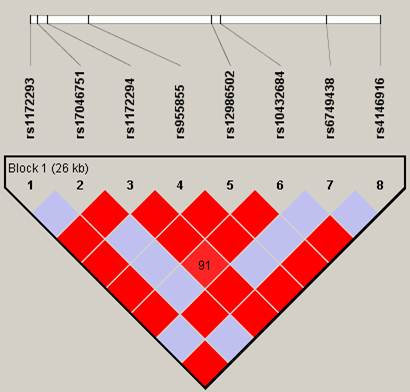
\includegraphics[height=170pt]{RBJ.jpg}

            }
            \hspace{10pt}
            \subfloat[Gene GPRC5B]{
                \centering
                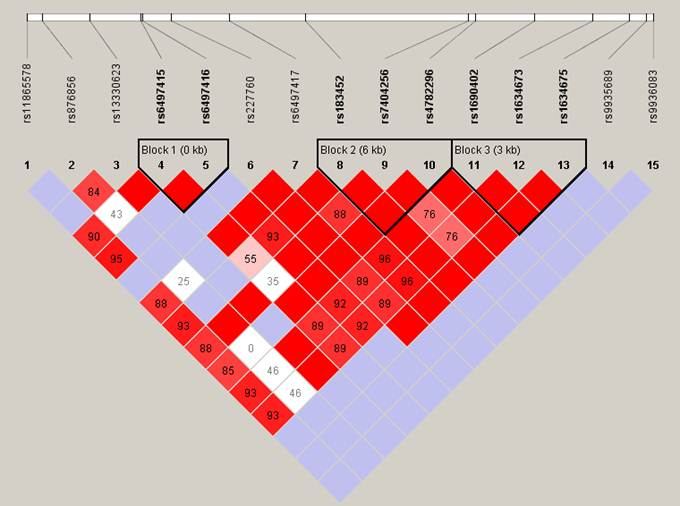
\includegraphics[height=170pt]{GPRC5B.jpg}
            }
            \caption{LD patten of the two genes}
        \end{figure}

        \begin{table}[htbp]
            \centering
            \caption{LD and MAF information for Gene RBJ and GPRC5B}
            \subfloat[Gene RBJ]{
                \begin{minipage}[b]{0.4 \textwidth}
                    \begin{tabular}{c|cc}
                        \toprule
                        SNP	&	LD			&	MAF			\\
                        \midrule
                        1	&	0.588	(	H	)&	0.115	(	R	)\\
                        2	&	0.159	(	L	)&	0.062	(	R	)\\
                        3	&	0.126	(	L	)&	0.482	(	C	)\\
                        4	&	0.588	(	H	)&	0.115	(	R	)\\
                        5	&	0.588	(	H	)&	0.115	(	R	)\\
                        6	&	0.565	(	H	)&	0.119	(	R	)\\
                        7	&	0.159	(	L	)&	0.062	(	R	)\\
                        8	&	0.588	(	H	)&	0.115	(	R	)\\
                        \bottomrule
                    \end{tabular}
                \end{minipage}
            }
            \hspace{10pt}
            \subfloat[Gene GPRC5B]{
                \begin{minipage}[b]{0.4 \textwidth}
                    \begin{tabular}{c|cc}
                        \toprule
                        SNP	&	LD			&	MAF			\\
                        \midrule
                        1	&	0.186	(	H	)&	0.146	(	R	)\\
                        2	&	0.05	(	L	)&	0.066	(	R	)\\
                        3	&	0.065	(	L	)&	0.044	(	R	)\\
                        4	&	0.194	(	H	)&	0.195	(	R	)\\
                        5	&	0.197	(	H	)&	0.143	(	R	)\\
                        6	&	0.136	(	L	)&	0.159	(	R	)\\
                        7	&	0.259	(	H	)&	0.46	(	C	)\\
                        8	&	0.262	(	H	)&	0.336	(	C	)\\
                        9	&	0.23	(	H	)&	0.482	(	C	)\\
                        10	&	0.206	(	H	)&	0.371	(	C	)\\
                        11	&	0.285	(	H	)&	0.394	(	C	)\\
                        12	&	0.285	(	H	)&	0.394	(	C	)\\
                        13	&	0.138	(	L	)&	0.155	(	R	)\\
                        14	&	0	(	L	)&	0.004	(	R	)\\
                        15	&	0	(	L	)&	0.005	(	R	)\\
                        \bottomrule
                    \end{tabular}
                \end{minipage}
            }
        \end{table}
        
        Table 1 is a brief summary of the two genes. For gene RBJ, it has 8 SNPs, the left table shows the SNPs feature in RBJ. The right table shows the information for SNP in Gene GPRC5B which has 15 SNPs. For each SNP, two measurements are listed. One is the LD pattern, which shows the average correlation between one SNP and other SNPs in the same gene. The other measurement is minor allele freq (MAF). The reason that we focus on LD and MAF is that we think these two would be the main factors affecting the final result. conditions. To convince our result analysis, I transform the original quantitative LD and MAF data into binary data: SNP is defined to have high LD (H) with other SNPs if its average LD $>$ 0.18, otherwise it has a low LD (L). A SNP labeled with C mean it is a common SNP which has MAF $>0.2$ and R means it has a MAF $\leq 0.2$.

        \begin{table}[htbp]
            \centering
            \caption{Simulation models}
            \begin{tabular}{c|l}
                \toprule
                Model 1 & $Y =\beta\times (SNP^A_1\times SNP^B_1+SNP^A_2\times SNP^B_2)+e$  \\
                Model 2 & $Y =\beta\times (SNP^A_1+SNP^B_1)+e$\\
                Model 3 & $Y =\beta\times (SNP^A_1\times SNP^A_2+SNP^B_1\times SNP^B_2)+e$\\
                \bottomrule
            \end{tabular}            
        \end{table}

        In the simulation studies, we try different models to test the performance of our method and other methods. Following is how we generate the simulated data. First we download the genotype of RBJ and GPRC5B from HapMap(http://hapmap.ncbi.nlm.nih.gov/) as a gene bank. Then we simulated the genotype person by person. For the $ith$ individual, we random picked one person's genotype in the gene bank as the $ith$ individual's genotype. After that, we picked one or two SNPs(depends on the model) to generate the phenotype according to different models(shown in Table 2). Here, $SNP^i_j$ stands for the $jth$ SNP from Gene $i$, $e$ is an error term follows normal distribution with mean 0 and variance 1. $\beta$ is a scale parameter which control the power. We tune $\beta$ so that the power of different SNP sets are distinguishable. 

        Here are the results from our simulation study. First is the model 1, it is a typical interaction model. And the interaction only occurs between genes. For each Gene, I will pick 2 SNPs as the casual SNPs, and assign a interaction effect to the product of two casual SNPs from different genes, then I add the two interaction effect to generate the phenotype. In the figure, the x axis is the method, we compare our method with widely used PCA and PLS, the y axis is the power, the higher, the better. From the result, we can see that in most cases, our method is better than PCA and PLS. And the bigger the minor allele freq. that is more common SNP show up, the larger the power, and the higher LD, the larger the power is.But when the casual SNP is in Low LD, and the minor allele freq is quite small, our method does not perform as good as the other two methods.We also simulate some other models like additive model and within gene interaction model, both the results show that our method has a better ability to detect the interaction, i.e., has more power. And also, just like the conclusion from additive model, when the casual SNP is in Low LD and the minor allele freq is low, our method did not perform well.
      
        \begin{figure}[htbp]
            \centering
            \subfloat[model 1]{
                \centering
                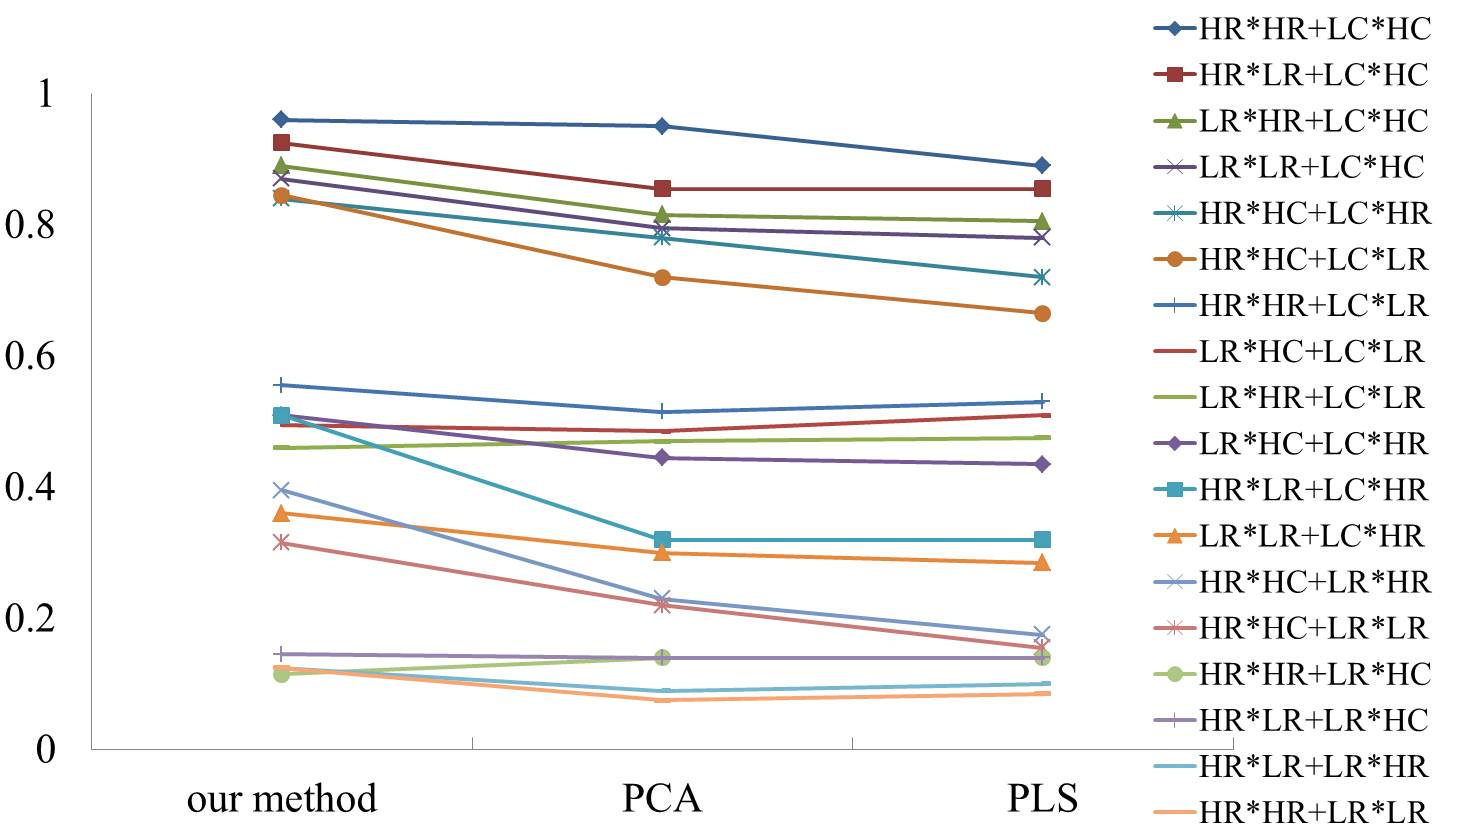
\includegraphics[height=170pt]{model1.jpg}
            }
            \hspace{10pt}
            \subfloat[model 2]{
                \centering
                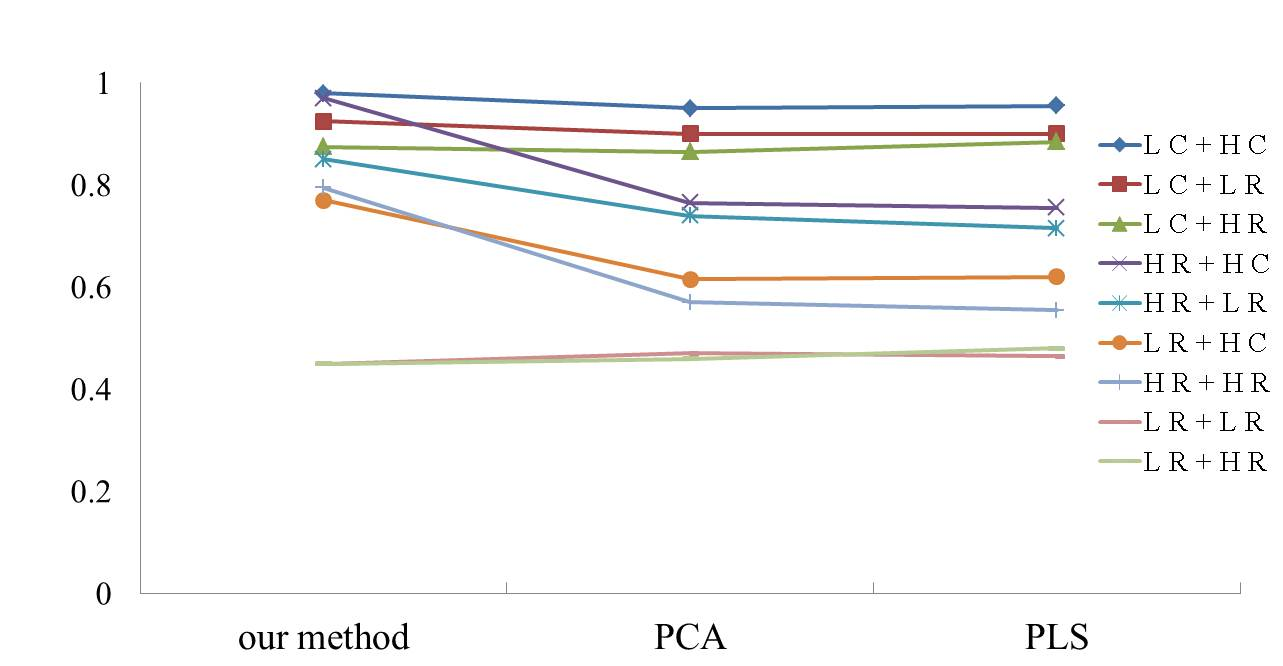
\includegraphics[height=170pt]{model2.jpg}
            }
            \hspace{10pt}
            \subfloat[model 3]{
                \centering
                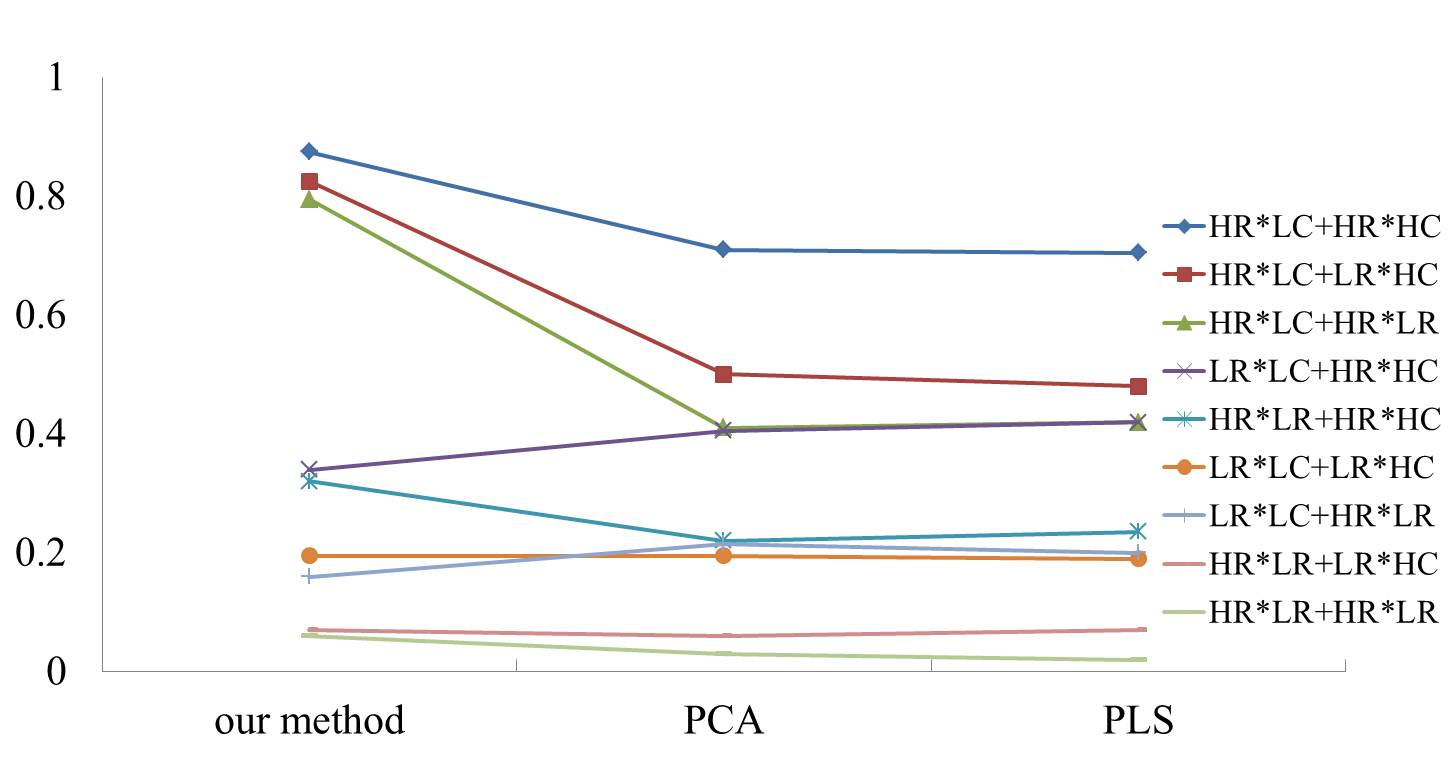
\includegraphics[height=170pt]{model3.jpg}
            }
            \caption{result for models}
        \end{figure}  


    \section{Appendix}

        \subsection{Score test for joint test and interaction test}

            For the model:
            \begin{equation*}
                Y=X\gamma+G_A+G_B+G_{AB}+e
            \end{equation*}

            Define $\theta=\{\sigma,\tau_A,\tau_B,\phi\}$, the REML log-likelihood function $L(\theta)$ for the whole data set is:
            \[
                L(\theta)=-\frac{1}{2}\bigg[\log|V|+\log|\X'V^{-1}\X|+\Y'P\Y\bigg]
            \]

             where $V=Var(Y)=\tau_AS_A+\tau_BS_B+\phi S_{AB}+\sigma I$ is the marginal variance of $\Y$ and $P=V^{-1}-V^{-1}\X(\X'V^{-1}\X)^{-1}\X'V^{-1}$ is the projection matrix for the model.

            Simple algebra shows that the score statistic under $H_0:\tau_A=\tau_B=\phi=0$ is

            \[
                U_{\sigma^2_b}=\frac{\partial L(\sigma^2_b,\sigma^2_e)}{\partial \sigma^2_b}\bigg|_{\sigma^2_b=0}=\frac{1}{2}[\Y'P_0SP_0\Y-tr(P_0S)]
            \]

            where the $P_0=\sigma^{-2}_e(I-\X(\X'\X)^{-1}\X')=\sigma^{-2}_eQ$. It is easy seen that $E(U_{\sigma^2_b})=0$ under $H_0^*$ and when $\sigma^2_b>0$, $E(U_{\sigma^2_b})=\sigma^2_b\cdot tr(QSQS)/(2\sigma^4_e)$ which is a strictly increasing function. Therefore larger values of $U_{\sigma_b^2}$ provides stronger evidence against $H_0^*$. This suggests that the testing procedure should be one sided.

            If $\sigma_e^2$ is known, the second term in our test is a constant. Therefore using the score statistic is equivalent to using the first term of $U_{\sigma^2_b}$ (denoted by $T$):
            \[
                T=\frac{1}{2}\Y'P_0SP_0\Y=\frac{1}{2\sigma^4_e}\Y'QSQ\Y
            \]
            Since Q is projection matrix for $\X$, we can show that
            \[
                T=\frac{1}{2\sigma^4_e}\Y'QSQ\Y=\frac{1}{2\sigma^4_e}(\Y-\X\mu)'QSQ(\Y-\X\mu)\sim\sum_{i=1}^c\lambda_i\chi^2_1
            \]
            where $\lambda_i$ is the ordered nonezero eigenvalues of teh matrix $QSQ/(2\sigma^2_e)$

            If $\sigma^2_e$ is unknown, we can replace $\sigma^2_e$ by $\hat{\sigma^2_e}$ using
            \[
                \hat{\sigma^2_e}=\frac{\Y'Q\Y}{N-1}
            \]

        \subsection{EM algorithm to estimate $\tau_A$, $\tau_B$ and $\sigma$}
            The model under the null hypothesis os $\phi=0$ is
            \[
                Y=X\gamma+G_A+G_B+e
            \]

            Y: $N\times1$ matrix, records trait value.

            X: $N\times p$ matrix, records the covariant.

            $\gamma$: $p\times 1$, the effect of covariant.

            $G_A$: the gene effect for Gene A, treated as an random effect. $G_A\sim N(0, \tau_AS_A)$, $S_A$ is the similarity matrix which records the genetic similarity between individuals.

            $G_B$: the gene effect for Gene B, also treated as an random effect. $G_A$ and  $G_B$ are assumed to be independent.

            $e$: $N\times1$ matrix,  the error term. $e\sim N (0, \sigma I)$.

            Define $U=A^TY$ with the restriction that $A^TA=I_{N-p}$ and $AA^T=I-P_X$.

            It is easy to find out that : $E(U)=0$ and $Var(U)=A^TVA$ where $V=Var(Y)=\tau_AS_A+\tau_BS_B+\sigma I$.

            \[ \begin{split}
                Cov(U,G_A)=& Cov(A^TX\gamma+A^TG_A+A^TG_B+A^Te,G_A)\\
                          =& Cov(A^TG_A,G_A)\\
                          =& A^TCov(G_A,G_A)\\
                          =&\tau_AA^TS_A
            \end{split}\]

            In the same way, we have$Cov(U,G_B)=\tau_BA^TS_B$ and $Cov(G_A,G_B)=0$ since they are independent.

            Therefore, the joint distribution of $(U,G_A,G_B)^T$ is
            \[
                \begin{pmatrix} U\\G_A\\G_B \end{pmatrix} \sim MN \begin{pmatrix} \mu=\begin{pmatrix} 0\\0\\0 \end{pmatrix},\quad \Sigma=\begin{pmatrix} A^TVA&\tau_AA^TS_A&\tau_BA^TS_B\\ \tau_AS_AA&\tau_AS_A&0\\\tau_BS_BA&0&\tau_BS_B \end{pmatrix} \end{pmatrix}
            \]

            so we can have the following conditional mean and variance,
            \begin{enumerate}
                \item the conditional mean and variance for $U$ are
                    \[\begin{split}
                        E(U|G_A,G_B)=&A^T(G_A+G_B)\\
                        Var(U|G_A,G_B) = & \sigma I_{N-p}
                    \end{split}\]
                \item the conditional mean and variance for $G_A$, since $Cov(G_A,G_B)=0$
                    \[\begin{split}
                        E(G_A|G_B,U)=&E(G_A|U)\\
                                                   =&\tau_AS_AA(A^TVA)^{-1}A^TY\\
                        Var(G_A|G_B,U)=&Var(G_A|U)\\
                                                       =&\tau_AS_A-\tau_A^2S_AA(A^TVA)^{-1}A^TS_A
                    \end{split}\]
                    Simple algebra shows that $A(A^TVA)^{-1}A^T=P=V^{-1}-V^{-1}X(X^TV^{-1}X)^{-1}X^TV^{-1}$, so that
                    \[\begin{split}
                        E(G_A|G_B,U)=&\tau_AS_APY=g_A\\
                        Var(G_A|G_B,U)=&\tau_AS_A-\tau_A^2S_APS_A=v_A
                    \end{split}\]
                \item Similarly, the conditional mean and variance for $G_B$ are
                     \[\begin{split}
                        E(G_B|G_A,U)=&\tau_BS_BPY=g_B\\
                        Var(G_B|G_A,U)=&\tau_BS_B-\tau_B^2S_BPS_B=v_B
                    \end{split}\]
            \end{enumerate}

            Define $\theta=\{\sigma,\tau_A,\tau_B\}$, according to the EM algorithm, we need to first compute the $\log L(\theta^{(t)}|U,G_A,G_B)$,
            \[\begin{split}
                \log L(\theta^{(t)}|U,G_A,G_B)=&f(U,G_A,G_B|\theta^{(t)})\\
                                                                         =&\log f(U|G_A,G_B,\theta^{(t)})+\log f(G_A|\theta^{(t)})+\log f(G_B|\theta^{(t)})
            \end{split}\]

            Since $S_A$ and $S_B$ are singular, we have,
            \[
                f(G_A)=\dfrac{1}{((2\pi)^{rank(S_A)}|\tau_AS_A|_+)^{\frac{1}{2}}}\exp\Big (-\dfrac{1}{2}G_A^T(\tau_AS_A)^-G_A\Big)
            \]

            where $|\tau_AS_A|_+$ is the Pseudo-Determinant, and $(\tau_AS_A)^-)$ is the Generalized inverse.

            Define $rank(S_A)=q_A$, $rank(S_B)=q_B$, we have,
            \[\begin{split}
                f(G_A)=&\dfrac{1}{((2\pi)^{q_A}\tau_A^{q_A}|S_A|_+)^{\frac{1}{2}}}\exp\Big (-\dfrac{1}{2\tau_A}G_A^T(S_A)^-G_A\Big)\\
                f(G_B)=&\dfrac{1}{((2\pi)^{q_B}\tau_B^{q_B}|S_B|_+)^{\frac{1}{2}}}\exp \Big(-\dfrac{1}{2\tau_B}G_B^T(S_B)^-G_B\Big)
            \end{split}\]

            therefore,

            \[\begin{split}
               \log f(G_A)=&constant -\dfrac{q_A}{2}\log \tau_A-\dfrac{1}{2}\log(|S_A|_+)-\dfrac{1}{2\tau_A}G_A^TS_A^-G_A\\
               \log f(G_B)=&constant -\dfrac{q_B}{2}\log \tau_B-\dfrac{1}{2}\log(|S_B|_+)-\dfrac{1}{2\tau_B}G_B^TS_B^-G_B\\
               \log f(U|G_A,G_B) =& constant-\dfrac{N-p}{2}\log\sigma-\dfrac{1}{2\sigma}\Big[(Y-G_A-G_B)^T(I-P_X)(Y-G_A-G_B)   \Big]
            \end{split}\]

            EM algorithm treats $G_A$ and $G_B$ as missing values. So instead of estimating $G_A$ and $G_B$ and then plugging them into the $\log L$, EM algorithm calculate the expectation of $\log L$ given $U$ and $\theta^{(t-1)}$, then based on $E(\log L|U,\theta^{(t-1)})$, $\theta^{(t)}$ are calculated by taking partial derivative.

            \[
                E\Big(\log L\Big|U,\theta^{(t-1)}\Big)=E\Big(\log f(G_A)\Big|U,\theta^{(t-1)}\Big)+E\Big(\log f(G_B)\Big|U,\theta^{(t-1)}\Big)+E\Big(\log f(U|G_A,G_B)\Big|\theta^{(t-1)}\Big)
            \]

            It is easy to find out that to estimate $\tau_A^{(t)}$, we just need to consider $E\Big(\log f(G_A)\Big|U,\theta^{(t-1)}\Big)$, so let
            \[\frac{\partial E\Big(\log f(G_A)\Big|U,\theta^{(t-1)}\Big)}{\partial\tau_A}=0\]
            we have,
            \[
                -\dfrac{q_A}{2\tau_A}+\dfrac{1}{2\tau_A^2}E\Big(G_A^TS_A^-G_A\Big|U,\theta^{(t-1)}  \Big)=0
            \]

            \[
                E\Big(G_A^TS_A^-G_A\Big|U,\theta^{(t-1)} \Big)=\big(g_A^{(t-1)}\big)^TS_A^-g_A^{(t-1)}+tr(S_A^-v_A^{(t-1)})
            \]
            plugging the expression of $g_A^{(t-1)}$ and $v_A^{(t-1)}$, finally we have
            \[
                \tau_A^{(t)}=\tau_A^{(t-1)}+\dfrac{[\tau_A^{t-1}]^2}{q_A}\Big[Y^TPS_APY-tr(S_AP) \Big]
            \]
            In the same way, we can estimate $\tau_B^{(t)}$ by
            \[
                \tau_B^{(t)}=\tau_B^{(t-1)}+\dfrac{[\tau_B^{t-1}]^2}{q_B}\Big[Y^TPS_BPY-tr(S_BP) \Big]
            \]
            To estimate $\sigma^{(t)}$, we just need to consider $E\Big(\log f(U|G_A,G_B)\Big|\theta^{(t-1)}\Big)$, so the final expression of $\sigma^{(t)}$ is
            \[
                \sigma^{(t)}=\dfrac{1}{N-p}\Big\{\Big[(Y^*)^T(I-P_X)Y^*\Big] + tr\Big[(I-P_X)\Big(\tau_A^{(t-1)}S_A-(\tau_A^{(t-1)})^2S_APS_A+\tau_B^{(t-1)}S_B-(\tau_B^{(t-1)})^2S_BPS_B\Big)\Big]         \Big\}
            \]
        where $Y^*=Y-\tau_A^{(t-1)}S_APY-\tau_B^{(t-1)}S_BPY$

\end{document} 